\documentclass{article}
\usepackage{amsmath}
\usepackage{graphicx}
\usepackage{url}

\title{LaTeX CS-E4004}
\author{Henrik Heinonen}
\date{\today}

\begin{document}
\maketitle

%Nothing else on first page
\newpage


\tableofcontents
\newpage

\section{Maths}

\subsection{Pythagorean theorem}

\begin{equation*}
    a^2 + b^2 = c^2
\end{equation*}
\textbf{a} and \textbf{b} represent lenght of sides for triangle and \textbf{c} is length of the hypotenuse.

\begin{center}
    \begin{equation*}
        f(x) = x^2
    \end{equation*}
\end{center}

\section{Figure}

\begin{figure}[h!]
    \centering
    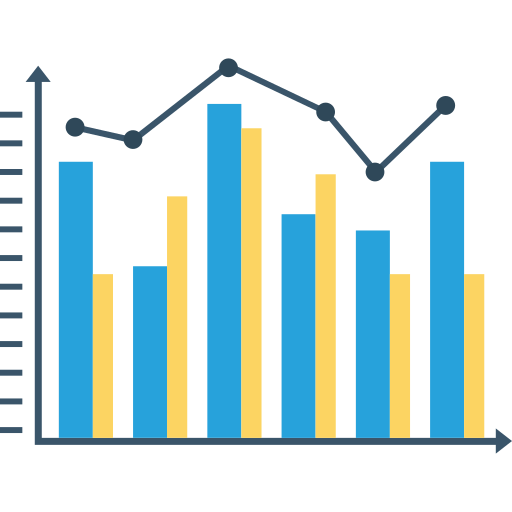
\includegraphics[width=\linewidth]{graph.png}
\end{figure}
Example graph \cite{WEBSITE:1}

\newpage
\bibliography{main}
\bibliographystyle{ieeetr}

\end{document}